\documentclass[border=10pt,varwidth]{standalone}
\usepackage{tikz}

\newcommand*{\vecref}[2]{\ensuremath{^#2 \vec{#1}}}
\newcommand*{\pref}[2]{\ensuremath{^#2{#1}}}
\newcommand*{\refsys}[1]{\ensuremath{\{#1\}}}
\newcommand*{\refframe}[4]{%
\draw[->,  #4] (0,0) to (#1, 0) node[right]{#2};
\draw[->,  #4] (0,0) to (0, #1) node[above]{#3};} 

\begin{document}
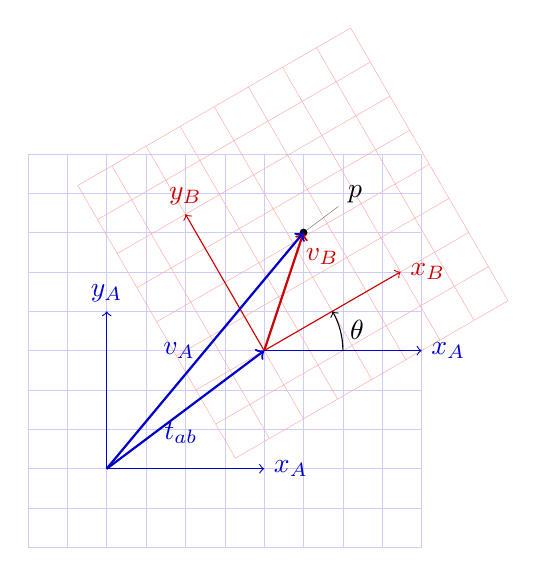
\begin{tikzpicture}[scale=0.5]

\def\xxa{5}
\def\yya{6}
\def\bx{4}
\def\by{3}
\def\thth{30}
\pgfmathsetmacro{\cth}{cos(\thth)}
\pgfmathsetmacro{\sth}{sin(\thth)}
\pgfmathsetmacro{\xxb}{\cth*(\xxa-\bx) + \sth*(\yya-\by)}
\pgfmathsetmacro{\yyb}{-\sth*(\xxa-\bx) + \cth*(\yya-\by)}

\draw[step=1cm, blue!20!white, very thin] (-2, -2) grid (8,8);

\refframe{4}{$x_A$}{$y_A$}{blue!80!black}

\begin{scope}[xshift = \bx cm, yshift=\by cm, rotate=\thth]
  \draw[step=1cm, red!30!white, very thin] (-2, -2) grid (6,6);
  \refframe{4}{$x_B$}{$y_B$}{red!80!black}
  \node[black, pin={[black] 30:{$p$}}, circle, fill, inner sep=1pt] at (\xxb cm, \yyb cm) {};

  \draw[thick, red!80!black,->] (0,0) -- node[pos=0.8, right] {$v_B$} (\xxb cm, \yyb cm); 
\end{scope}

  \draw[thick, blue!80!black,->] (0,0) -- node[pos=0.3, right] {$t_{ab}$} (\bx cm, \by cm); 
  \draw[thick, blue!80!black,->] (0,0) -- node[pos=0.5, left] {$v_{A}$} (\xxa cm, \yya cm); 

  \draw[blue!80!black, thin, ->] (\bx cm, \by cm) -- ++(4cm, 0) node[right] {$x_A$};
  \draw[->] (\bx cm, \by cm) ++ (2cm, 0) arc[radius=2cm, start angle=0, end angle=\thth] node[right, pos=0.5] {$\theta$};

%\node[red!80!black, pin=30:{}, circle, fill, inner sep=1pt] at (\xxa cm, \yya cm) {};
\end{tikzpicture}
\end{document}
